\headline{{\textbf{\Large\sffamily Bonsai Roots:}}\\
          {\textbf{\large\sffamily Meet the Members of TWBC}}}
\label{2025-10-roots}
\noindent
In every edition of \emph{Bonsai Roots,} we take a break from pruning and potting to spotlight the members who bring our club to life.
Each story adds a branch to the growing canopy of TWBC. This month, we're delighted to introduce \textbf{John}!

\begin{itemize}
    \item \textbf{What's your name and where in the country do you live?}

    \emph{My name is John Mari and I live in Chiswick, London.}

    \item \textbf{What are your favourite species of tree and why?}

    \emph{I've always been drawn to maples — they're delicate, elegant, and constantly changing. The range of colours throughout the seasons is simply amazing.}

    \item \textbf{What aspect of bonsai do you enjoy?}

    \emph{For me, it's the shaping of a tree to match the image in your imagination. That creative moment when form begins to emerge from nature feels incredibly rewarding.}

    \item \textbf{What aspects of bonsai do you find most challenging?}

    \emph{Given that I'm new to bonsai — at the moment, all of it! Every stage feels like a lesson, but that's also part of the fun.}

    \begin{window}[%
        2,l,%
        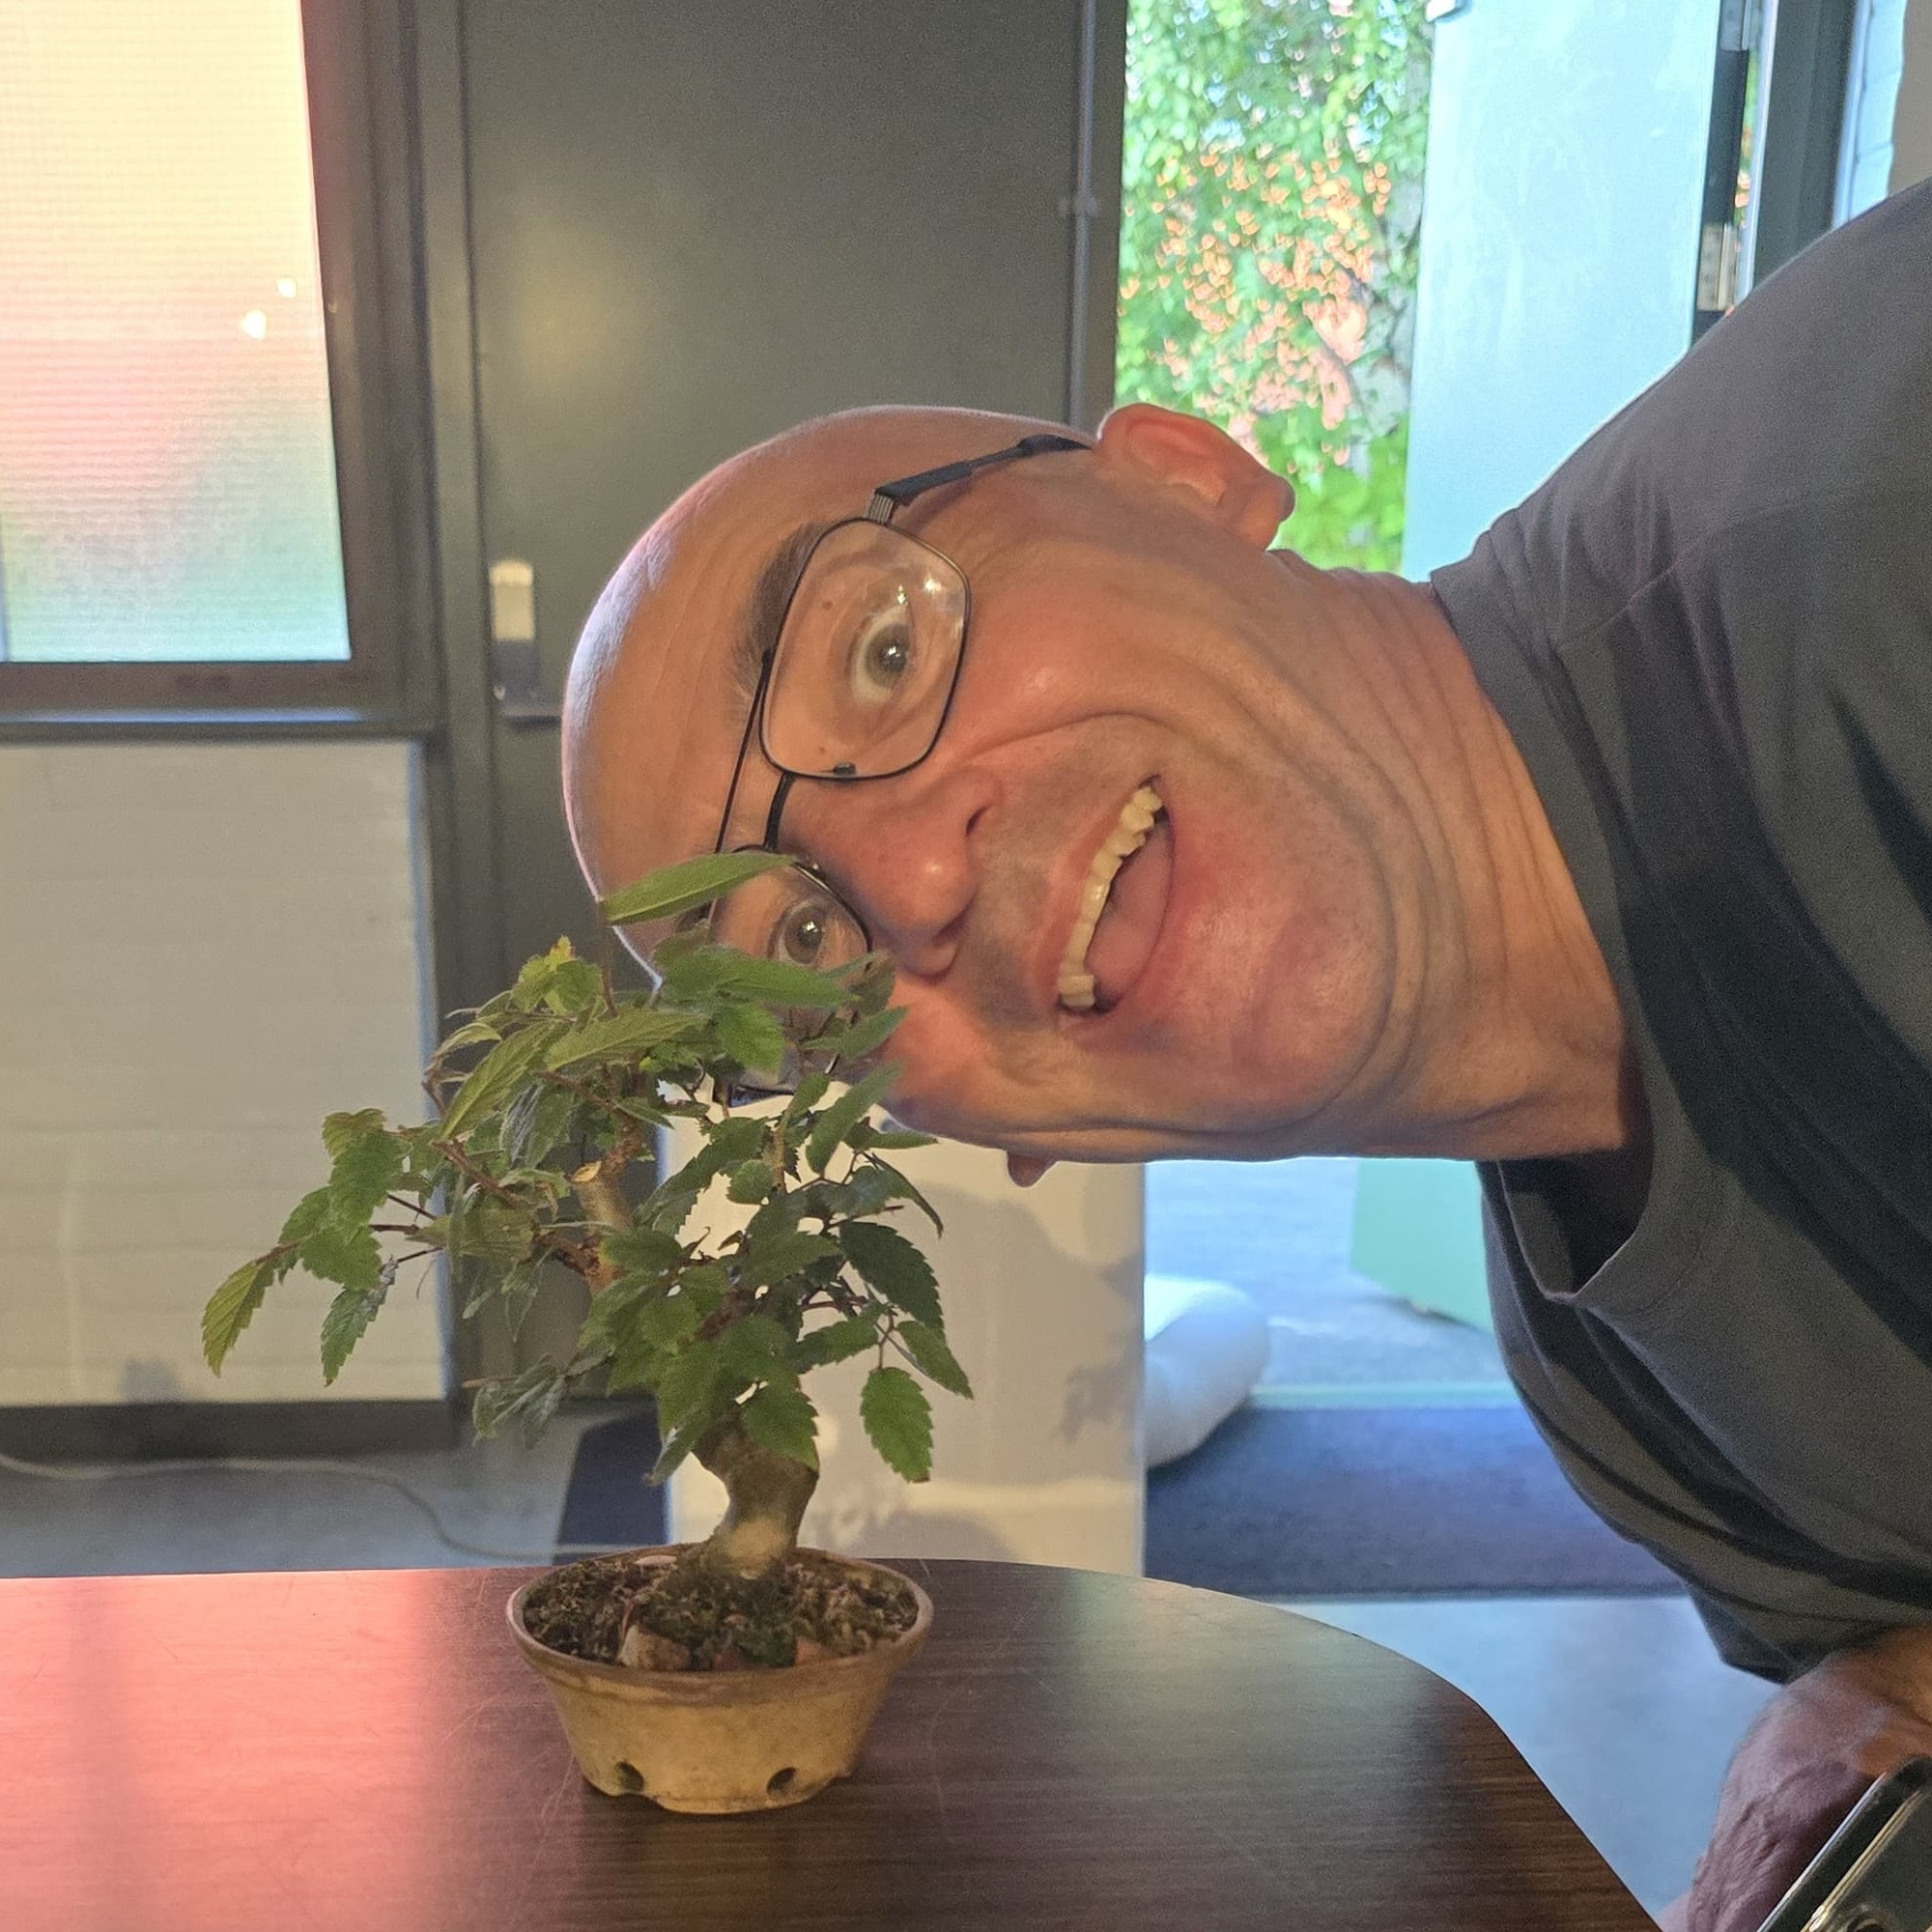
\includegraphics[width=1.0\columnwidth]{2025_10/res/roots_john_mari.jpeg},%
        \centerline{\emph{John photobombing his Tree of the Month contribution.}}%
    ]
    \end{window}
    \columnbreak

    \item \textbf{Who or what inspires you throughout your bonsai journey?}

    \emph{My friend Victoria — her knowledge, enthusiasm, and passion are truly infectious. She's been a big influence in helping me take my first steps into the hobby.}

    \item \textbf{How long have you been interested in keeping bonsai?}

    \emph{I've admired bonsai all my life, but it's only recently that I've actually started growing and shaping trees of my own.}

    \item \textbf{What stimulated your interest in bonsai?}

    \emph{Their beauty — there's something captivating about how a tree can express so much character in miniature form.}

    \item \textbf{If you could give someone new to bonsai any tips, what would it be?}

    \emph{Just start! You'll learn as you go, and every tree will teach you something new.}

    \item \textbf{Why do you enjoy being part of TWBC, and do you have any ideas or suggestions for the club's future?}

    \emph{The people — everyone is so friendly and welcoming. It's great to be part of a community where you can share ideas, learn, and laugh together.}

    \item \textbf{One word to describe what bonsai means to you?}

    \emph{Elegance.}

    \item \textbf{What are your future goals regarding your own trees and learning more about the hobby?}

    \emph{To see my trees grow and develop into the vision I have for them. I'd like to build patience and skill as they evolve, one season at a time.}

    \item \textbf{How would you like to see your bonsai journey progress in the future?}

    \emph{With enjoyment, creativity, and the hope of one day creating something beautiful that I can pass on to my son.}
\end{itemize}

John's bonsai path is just beginning, but his enthusiasm and curiosity already shine through --- along with that big smile behind the trees!
We look forward to seeing how his vision grows.
Who will we meet next time?
Stay tuned for more in \emph{Bonsai Roots}!

\begin{center}
    $\cdots$
\end{center}

\noindent
\emph{If you're a newer member and would like to feature in a future edition of Bonsai Roots, simply fill out the form at \href{https://forms.gle/quVXa4L8rhpnT5kr6}{this link}! We'd love to hear your story.}
\closearticle
\columnbreak
